\documentclass[oneside,12pt]{report}  

% the dimensions of the page
\textheight=9.25in \topmargin=-0.5in   %See note in Chapter 8 of Sample Report about "Page scaling" option in Adobe
\textwidth=6.0in
\oddsidemargin=0.3in
\evensidemargin=0.3in  % Needed to balance even and odd pages in twoside print copy


% Useful packages
\usepackage{dtklogos}
\usepackage{amsmath}
\usepackage{bm}
%\usepackage[colorlinks=true,pagebackref,linkcolor=blue]{hyperref}
\usepackage{amsfonts}
\usepackage{amsthm}
\usepackage{amsmath}
\usepackage{algorithm}
\usepackage{algorithmic}
\usepackage{graphicx, subfigure}
\usepackage{caption}
\usepackage{excludeonly}

\usepackage{graphicx} 

%\usepackage{doc}
%% Following sets up logic and formatting for conditional twoside copying
%\usepackage{ifthen, color, fancyvrb}
%\usepackage{nextpage}\pagestyle{plain}
%\newcommand\myclearpage{\cleartooddpage
%  [\thispagestyle{empty}]
%  }

\DeclareMathOperator*{\argmin}{arg\ min}
\DeclareMathOperator*{\sign}{sign}

% Note special alternative codes for using TWO bibliographies; see cautionary note in
\DeclareGraphicsExtensions{ps,eps,PNG,png}

% Theorem-like command definitions:
\newtheorem{theorem}{Theorem}[chapter]
\newtheorem{lemma}{Lemma}[chapter]
\newtheorem{definition}{Definition}  % Note, this italicizes everything

% Print the chapter and sections in the toc
\setcounter{tocdepth}{1}

% Specify which files to typeset for this run (note that overall pagination is preserved)
%\includeonly{chapter1, chapter2}
% Specify which files NOT to typeset for this run (note that overall pagination is preserved)
%\excludeonly{}

% Groundwork for allowing double-sided copying with blank versos
\def\prefacesection#1{
\chapter*{#1}
\addcontentsline{toc}{chapter}{#1}
}

\begin{document}


\def\thefootnote{\fnsymbol{footnote}}

\thispagestyle{empty}

% The numbers below controls the amount of space between the following sections
\def\shiftdowna{0.32in}  % Adjust for balance
\def\shiftdownb{0.22in}  % Adjust for balance

% Set up the boiler plate at the top of the page

\begin{center}
\textbf{{\large Mathematical Modeling and Consulting }}\\

\vspace \shiftdowna

\includegraphics[width=0.5\textwidth]{jhu.png}\\

% Home Department
\vspace \shiftdowna
\underline {Sponsor}\\ 
\vspace{5pt}
\textbf{\large Eastern Interconnection States Planning Council} \\
\vspace\shiftdowna
\textbf{{Progress Report}}

% TITLE
\vspace \shiftdowna
\textbf{{\Large The Value of Co-optimization in Electric Power Planning}}

% STUDENTS
\vspace{0.35in}
\underline {Team Members}\\
\vspace{5pt}
\text{Jonathan Ho}, \texttt{jho19@jhu.edu}\\
\vspace{5pt}
\text{Jordan Mandel}, \texttt{jmande10@jhu.edu}\\
\vspace{5pt}
\text{Yue Wu}, \texttt{ywu67@jhu.edu}\\
\vspace{5pt}
\text{Mengshu Wang}, \texttt{mwang53@jhu.edu}\\
\vspace{10pt}

% INSTRUCTOR
\vspace \shiftdownb
\underline {Academic Mentor} \\
\vspace{5pt}
\text{Dr.~N.~.H.~Lee}, Applied Mathematics and Statistics\\
\texttt{nhlee@jhu.edu}

% Consultants
%\vspace \shiftdownb 
%\underline {Consultant}\\
%\vspace{5pt}
%Jason Bourne\\

% DATE
\vspace \shiftdowna
Date: Last Complied on \today

\end{center}

\vfill  %Fill page to force following note to bottom
\footnoterule
\noindent \small{Any apparent association of this work to  the real EISPC is fictional, and the sole purpose of this work is a class exercise}

% Begin ABSTRACT
\ifthenelse{\boolean{@twoside}}{\myclearpage}{}
\prefacesection{Abstract}
Transmission planning is complex due to the large number of market participants, whose behavior and decisions are outside the control of the transmission planner. Current planning techniques which assume system variables outside of the control of the transmission planner excludes potentially lower cost solutions. Co-optimization is an improved modeling technique that allows a transmission planner to simultaneously model transmission planners along side generation planners.

% Begin ACKNOWLEDGMENTS
%\ifthenelse{\boolean{@twoside}}{\myclearpage}{}
%\prefacesection{Acknowledgments}

% Table of contents, List of Figures, and List of Tables.
\ifthenelse{\boolean{@twoside}}{\myclearpage}{}
\tableofcontents

\ifthenelse{\boolean{@twoside}}{\myclearpage}{}
\listoffigures


%\ifthenelse{\boolean{@twoside}}{\myclearpage}{}
%\listoftables


\renewcommand{\thefootnote}{\arabic{footnote}}
\setcounter{footnote}{0}

\ifthenelse{\boolean{@twoside}}{\myclearpage}{}

\chapter{Introduction}
The Eastern States Interconnection Planning Council (EISPC) is a collaborative organization for the Eastern AC Interconnection. Through it, state and federal organizations work to improve coordination  amongst states and to develop better planning tools. EISPC facilitates interconnection wide planning decisions that will improve the robustness of the interconnection by making use of industry leading tools and expertise. 

\chapter{Problem Statement}
Using a co-optimization process that models the behavior of generators and transmission operators could reduce total system costs for both market participants.
There are two major issues that confound interconnection wide transmission planning efforts. The first is that organization of utilities transmission organizations in the United States. Traditionally in the utilities were vertically integrated publicly regulated monopolies. This allowed a utility to coordinate investments in generation and transmission. Under this type of organization there is little incentive for a utility to invest in transmission with a neighboring utility as their monopoly guaranteed that a utility could always afford to build the necessary generation capacity within their own network.

During the 90s deregulation of the power sector made it possible to break a utilities monopoly on generation. Under this model transmission would remain a monopoly operated by an independent system operator (ISO). ISOs operate a transmission network for a region and are nearly all non-profit. Generation is no longer a monopoly and utilities can either provide for themselves or buy from competitive independent generators. Under an ISO there is significantly more investment in transmission and interconnection as utilities will buy the cheapest available power in the system regardless of where it is produced. Making these interconnection decisions is complicated because the transmission planner, the ISOs, no longer coordinate with generation planers, utilities and independent producers.

An additional challenge to transmission planners is the expansion of renewable energy. Renewable generation has grown rapidly over the past decade and will continue to do so, with growth projections by the International Energy Agency in excess of 40\%, due to declining costs, government regulation, and economic incentives. \cite{IEA} In many cases the best quality renewable resources are located far from the areas of high demand, and would require significant investments in transmission to become viable. 

Currently the US electric network is made up of a mix of deregulated power pools and vertically integrated monopolies. Transmission planning is not preformed with appropriate considerations for the value of co-optimization. Under existing planning process transmission planning is preformed under the assumption that generation remains constant. Ignoring the generation planning process may result in the construction of lines that turn out to be unnecessary as well as limit the construction of inexpensive renewables. This will result in higher costs to all parties involved. This project will demonstrate that co-optimizing transmission investment decisions can reduce the total cost of building and operating an electric power system.

\chapter{Current Achievement}
The first stage of analysis has focused on computing and organizing the necessary inputs to allow the co-optimization model to run. The completed analysis has includes, existing generation technology, electricity demand profiles, and the aggregation of state RPS's to regions. 
\\For cases where parameters needed to be aggregated to regions population weighting was used. Population weighting is useful because, energy usage and population are highly correlated. County level population data from the 2010 US Census data and corresponding map files were downloaded. A table was generated using ArcGIS containing the state populations falling into each electric region. These populations were used as weights to aggregate the state level data on generation and RPS standards to regional levels for use with the model.
\\The installed generation capacity was calculated using data from the Energy Information Agency. For the purpose of the model power plant data from 2004 was used. The EIA power plant data was further broken down into more specific technologies using a database of existing power plants provided by BenTek. The installed generation capacity by technology was aggregated to region using population weighting.
\\While regional demand data was provided in the McCalley PSERC paper, the data was limited to base demand. To develop time series data on demand this was combined with the 2004 hourly load data reported by ISOs. For non ISO regions demand profiles were developed by using normalized load profiles from similar lattitudes, which tend to be highly correlated. These load profiles were time shifted to adjust for  when regions were in different time zones.
\\Regional RPSes aggregated by population weighting the state RPS standards. Two tables for RPSes were calculated to match with the second and third stage of the co-optimization model. The first table includes only RPS standards that come into effect before the year 2020. The second table includes all RPS standards that come into effect before the year 2030.


\chapter{Ongoing and Future Work} 
One required model parameters is still being gathered including the hourly availability of renewable resources. The availability of hourly wind and solar generation is currently being gathered from resources at NREL. The Wind data is available through the Western and Eastern Wind studies. Solar data is being calculated using PVWatts a program that models the behavior of solar panels.
\\The current focus of ongoing work is on the adaption of a co-optimization model specific to the 13 bus network used. A running model has been developed and executed in AIMMS. Additional work is required to verfiy model is properly formulated.
\begin{figure}[h] 
  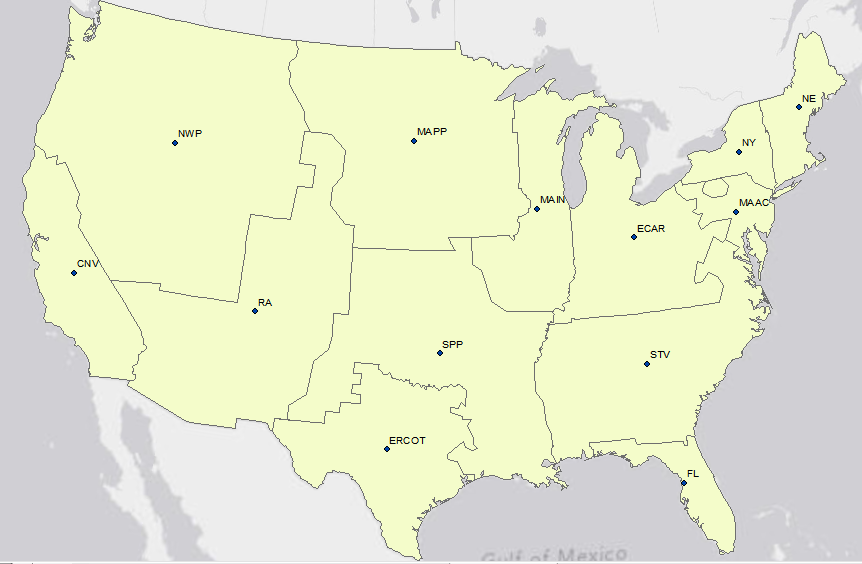
\includegraphics[width=6in]{map.png}
  \caption[Map of 13 buses]
   {Map of 13 buses}
\end{figure}
\\Future work that could be fulfilled are listed below:
\begin{itemize}
	\item Input parameter selection
	\item Baseline model need to be developed
	\item Analysis of model output using R
	\item R package
\end{itemize}
%\chapter{Conclusion}


\appendix
\ifthenelse{\boolean{@twoside}}{\myclearpage}{}

%\chapter{Lemmas}\label{Lemma}

\chapter{Glossary}\label{Glossary}

\vspace{12pt} 

\vspace{8pt}
\noindent {\bf Optimization}. A technique for finding optimal solutions subject to a set of constraints. 

\vspace{8pt}
\noindent {\bf Renewable Portfolio Standards}. A state may enact a requirement that a given percentage of their electricity demand must be met through renewable generation technologies. 
\ifthenelse{\boolean{@twoside}}{\myclearpage}{}
\chapter{Abbreviations}\label{Abbreviations}


\noindent EISPC. Eastern Interconnection States Planning Council

\vspace{5pt}

\noindent ISO. Independent System Operator


%\endinput

% Add your bibliography to Contents
\ifthenelse{\boolean{@twoside}}{\myclearpage}{\newpage}
\addtocontents {toc}{\protect \contentsline {chapter}{REFERENCES}{}}
\addcontentsline{toc}{chapter}{Selected Bibliography Including Cited Works}  

% Bibliography must come last.
\bibliographystyle{plain}
\renewcommand\bibname{Selected Bibliography Including Cited Works}
\nocite{*}  % List ALL references in your references, not just the ones cited in the text.
% This scheme automatically alphabetizes the Bibliography.
\bibliography{Biblio}
\end{document}
